\chapter[Lecture 3]{}\label{lec3}

\section*{A Thamizhavel}
\vskip -.5cm
\begin{figure}[H]
\centering
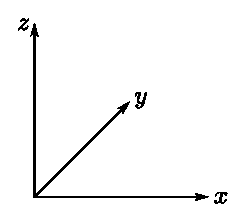
\includegraphics[scale=.8]{images/lecture3/fig1.eps}
\end{figure}

\section*{The Dimensional Lattice}

Seven lattice systems with 14 different lattice types.
\begin{longtable}{lcc}
\hline
\multicolumn{1}{c}{\bf System} & \multicolumn{1}{c}{\bf No. of lattices} & \multicolumn{1}{c}{\bf Cell axes and angles}\\[3pt]
\hline
Triclinic & 1 & $a_{1}\neq a_{2}\neq a_{3}$\\
          &   & $\alpha\neq \beta\neq \gamma$\\
Monoclinic & 2 & $a_{1}\neq a_{2}\neq a_{3}$\\
           &   & $\alpha=\gamma=90^{\circ}\neq \beta$\\
Orthorhombic & 4 & $a_{1}\neq a_{2}\neq a_{3}$\\
             & [Primitive, fc, bc, base centered] & $\alpha=\beta=\gamma=90^{\circ}$\\
Tetragonal & 2 & $a_{1}=a_{2}\neq a_{3}$\\
           &   & $\alpha=\beta=\gamma=90^{\circ}$\\
Cubic & 3 & $a_{1}=a_{2}=a_{3}$\\
      & [sc, fcc, bcc] & $\alpha=\beta=\gamma=90^{\circ}$\\
Trigonal & 1 & $a_{1}=a_{2}=a_{3}$\\
         &   & $\alpha=\beta=\gamma < 120^{\circ}\neq 90^{\circ}$\\
Hexagonal & 1 & $a_{1}=a_{2}\neq a_{3}$\\
          &   & $\alpha=\beta=90^{\circ}$\\
          &   & $\gamma=120^{\circ}$
\end{longtable}

Simple cubic systems: $\to$
{%\fontsize{9}{11}\selectfont
\begin{center}
\renewcommand{\arraystretch}{1.3}
\begin{tabular}{lccc}
\hline
\multicolumn{1}{c}{\bf Volume} & $\dfrac{\text{SC}}{a^{3}}$ & $\dfrac{\text{BCC}}{a^{3}}$ & $\dfrac{\text{FCC}}{a^{3}}$\\[7pt]
\hline
No. of lattic points per cell & 1 & 2 & 4\\[3pt]
No. of nearest neighbors & 6 & 8 & 12\\[5pt]
Nearest neighbor distance & $a$ & $\dfrac{\sqrt{3}a}{2}\simeq 0.866a$ & $\dfrac{a}{\sqrt{12}}\simeq 0.707a$\\[10pt]
Packing fraction & $\dfrac{\pi}{6}\newline =0.524$ & $\dfrac{\sqrt{3}}{8}\pi\newline =0.680$ & $\dfrac{\sqrt{2}}{6}\pi\newline =0.740$\\[7pt]
                 &                        & & [close packed]
\end{tabular}
\end{center}}\relax

\noindent
Primitive Vectors:-

\medskip
\noindent
SC: $\overrightarrow{a}_{1}=\widehat{x}a$; $\overrightarrow{a}_{2}=a\widehat{y}$; $\overrightarrow{a}_{3}=a\widehat{z}$

\medskip
\noindent
BCC : $\overrightarrow{a}_{1}=a\widehat{x}$; $\overrightarrow{a}_{2}=a\widehat{y}$; $\overrightarrow{a}_{3}=\dfrac{a}{2}\left[\widehat{x}+\widehat{y}+\widehat{z}\right]$

\medskip
\noindent
or, $\overrightarrow{a}_{1}=\dfrac{a}{2}\left[\widehat{x}+\widehat{y}-\widehat{z}\right]$; $\overrightarrow{a}_{2}=a\left[-\widehat{x}+\widehat{y}+\widehat{z}\right]$; $a_{3}=\dfrac{a}{2}\left[\widehat{x}-\widehat{y}+\widehat{z}\right]$

\medskip
\noindent
FCC : $\overrightarrow{a}_{1}=\dfrac{a}{2}\left[\widehat{x}+\widehat{y}\right]$; $\overrightarrow{a}_{2}=\dfrac{a}{2}\left[\widehat{y}+\widehat{z}\right]$; $\overrightarrow{a}_{3}=\dfrac{a}{2}(\widehat{x}+\widehat{z})$

\medskip
\noindent
Since \ \fbox{$\widehat{r}_{j}=\sum\limits^{3}_{i=1}x_{ij}a_{i}$}

\medskip

\begin{tabbing}
For BCC : \= $\left(\dfrac{1}{2} \ \dfrac{1}{2} \ \dfrac{1}{2}\right)$\\[8pt]
\phantom{For} FCC : \> $\left(\dfrac{1}{2} \ \dfrac{1}{2} \ 0\right)$; $\left(\dfrac{1}{2} \ 0 \ \dfrac{1}{2}\right)$; $\left(0 \ \dfrac{1}{2} \ \dfrac{1}{2}\right)$
\end{tabbing}

\section*{Index for Crystal Planes}

Plane defined by three non-colinear points and points are defined in terms of $a_{1}$, $a_{2}$, $a_{3}$.

Procedure:
\begin{itemize}
\item[(i)] Find intercepts of the plane on three axes (Primitive of non-primitive)

\item[(ii)] Take reciprocal of these numbers reduce them to make integers and written as $(hkl)$

\item[(iii)] (-ve) sign is written as bar $-2\Rightarrow \overline{2}$
\end{itemize}
Eg. If the intercepts are $3a_{1}$, $2a_{2}$, $2a_{3}$

\smallskip
Plane : $\left(\dfrac{1}{3} \ \dfrac{1}{2} \ \dfrac{1}{2}\right)\equiv (2 \ 3 \ 3)$ plane.

\smallskip
Cubic faces : $(1 \ 0 \ 0) \ (0 \ 1 \ 0) \ (0 \ 0 \ 1) \ (1 \ 1 \ 0) \ (1 \ 0 \ 1) \ (0 \ 1 \ 1) \ (1 \ 1 \ 1)$ etc.

\section*{Simple Crystal Structures}

Nacl : fcc \ Two fcc lattice displaced by $\left(\dfrac{1}{2} \ 0 \ 0\right)$

\medskip
\noindent
CsCl : BCC \ Two SC lattice displaced by $\left(\dfrac{1}{2} \ \dfrac{1}{2} \ \dfrac{1}{2}\right)$

\medskip
\noindent
Hexagonal Close Packed (HCP) : $ABAB....$

\medskip
\noindent
Note Cubic Close Packed : $ABC \ ABC \ ABC...$

\medskip
\noindent
Diamond Structure : fcc with basis $(0 \ 0 \ 0) \left(\dfrac{1}{4} \ \dfrac{1}{4} \ \dfrac{1}{4}\right)$

\medskip
\noindent
[4 out of 8 tetrahedral points are occupied]

\medskip
\noindent
Two fcc lattice displaced by $\left(\dfrac{1}{4} \ \dfrac{1}{4} \ \dfrac{1}{4}\right)$

\medskip
\noindent
{\bf Zinc Blend :} Diamond structure with $Zn$ in one fcc and $S$ in other fcc lattice.

\medskip
\noindent
{\bf Voids:} tetrahedral octahedral.
\begin{center}
\begin{tabular}{lcc}
\hline
{\bf FCC} & 8 & 4\\
\hline
Perovskite : & $ABC_{3}$ & \raisebox{-1.3cm}{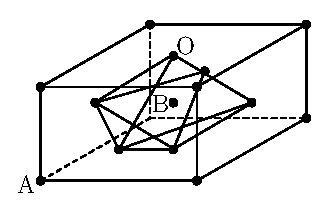
\includegraphics[scale=.8]{images/lecture3/fig2.eps}}\\
$K_{2}NiF_{4}$ : & &\\
\hline
\end{tabular}
\end{center}

\newpage

\section*{Layered structure}
\begin{figure}[H]
\centering
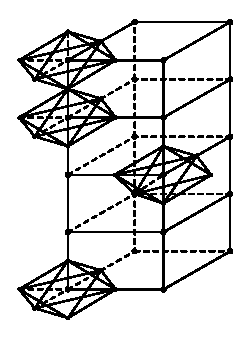
\includegraphics{images/lecture3/fig3.eps}
\end{figure}

\noindent
Ruddlesden - Popper Series : $A_{n+1}B_{n}X_{3n+1}$

\smallskip
\noindent
$K_{2}Nitu\to n=1$

\smallskip
\noindent
\textbf{\boldmath$AlB_{2}$ structure:}
\begin{figure}[H]
\centering
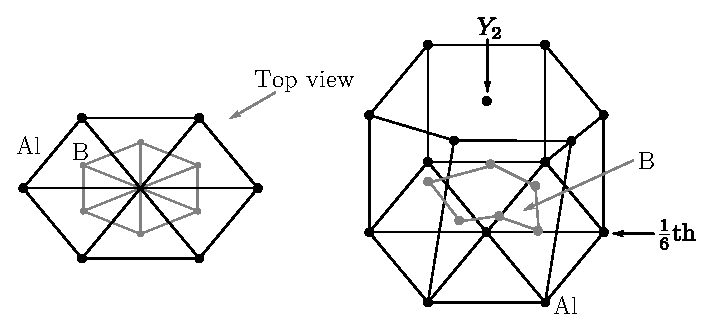
\includegraphics[scale=.8]{images/lecture3/fig4.eps}
\end{figure}

\smallskip
\noindent
\textbf{Cubic (3):} Simple Cubic/Primitive, bcc,fcc (centered lattice).
\begin{figure}[H]
\centering
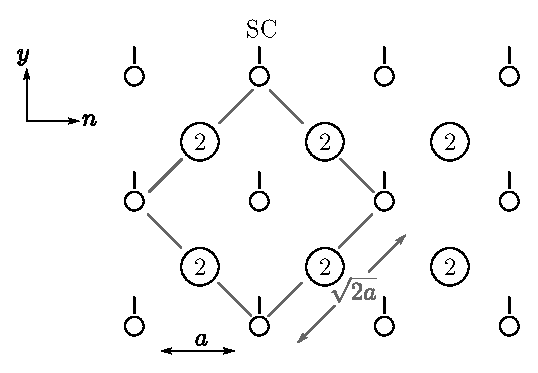
\includegraphics[scale=.8]{images/lecture3/fig5.eps}
\end{figure}
If (2) is at $(\frac{1}{2}\frac{1}{2}\frac{1}{2})$ it is BCC

The same lattice will become FCC if we define lattice with lattic constant $(\sqrt{2}a)$.

\medskip
\noindent
\textbf{Tetragonal (2):} Simple tetragonal (SC stretched along $c$), Centered tetragonal (BCC or FCC stretched along $c$).
\begin{align*}
\left.
\begin{array}{l}
c/a=1 \text{ (BCC) } \to \text{ stretched}\\
c/a=\sqrt{2} \text{ (FCC) } \to \text{ stretched}
\end{array}\right\}
\quad\text{centered lattice}
\end{align*}

\smallskip
\noindent
{\bf Orthorhombic (4) :}
\begin{figure}[H]
\centering
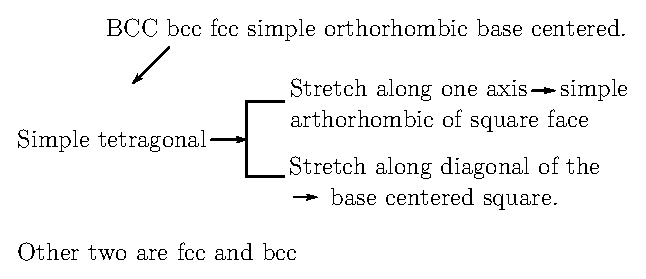
\includegraphics[scale=.8]{images/lecture3/fig7.eps}
\end{figure}
Other two are {\bf fcc} and {\bf bcc}.

\medskip
\noindent
{\bf Monoclimic (2) :} Distort rectangular face of orthorhombic cell to parallelogram $\to$ monoclinic

Both BCC and simple orthorhombic produces simple monoclinic

bcc and fcc $\to$ centered monoclinic structure.

\medskip
\noindent
{\bf 14 crystal lattices, 7 crystal systems}

\medskip
\noindent
{\bf Triclinic (1)} $\to$ Complete distortion $\to$ no angle is $90^{\circ}$.

This is the Bravais lattice with minimum symmetry.

\medskip
\noindent
{\bf Trigonal/Rhombohedral (1) :} Stretch the cube along body diagonal - lengths and angles are equal.

\medskip
\noindent
{\bf Hexagonal (1) :} Simple hexagonal.

** It is difficult to conclude if these are the only distict cases possible. However, we can safely state, the crystal lattices found so far fall within these categories.
